\documentclass{article}
\usepackage[utf8]{inputenc}
\usepackage{hyperref}
\usepackage{amsmath}
\usepackage{amsfonts}
\usepackage{graphicx}


\title{SPhO Ten Year Series (TYS) with Solutions: 2018 Questions}
\author{
    Solutions available on Victoris\\
    \texttt{victoris.org}
    % new collaborators add your name and contact here!
}

\date{\today}

\begin{document}
\maketitle

\section{2018 (1.5h for Q1-5, 1.5h for Q6-9)}
\subsection{Question 1}
1. A particle $\mathrm{X}$ is projected with speed $v$ in a direction which makes an angle of $30^{\circ}$ from the horizontal. When this particle reaches the highest point of its trajectory, another particle $\mathrm{Y}$ is dropped from the roof of a tall building. The two particles collide at the base of the building. The particle $\mathrm{Y}$ takes a time of $0.17 \mathrm{~s}$ to fall a $5.0 \mathrm{~m}$ tall window in the building. The base of the window is $50.0 \mathrm{~m}$ above the ground. Ignore the effect of air resistance, find \\
i) the height of the building; [4] \\
ii) the value of $v$; [4] \\
iii) the distance of the point of projection of $X$ from the foot of the building. [2]

\subsection{Question 2}
2. A horizontal platform vibrates with simple harmonic motion in the horizontal direction with a period of $2.0 \mathrm{~s}$. A small object placed on the platform starts to slide when the amplitude of vibration reaches $0.4 \mathrm{~m}$. \\
i) Calculate the coefficient of static friction between the object and the platform. [5] \\
ii) The platform now excutes vertical simple harmonic motion with a period of $1.5 \mathrm{~s}$. What is the maximum amplitude of the motion if the object were to be in contact with the plate throughout the motion? [5]

\subsection{Question 3}
3. Consider a gas with molecular mass $m$ in a constant gravitational field $\mathbf{g}$. \\
i) Write down an equation relating a small change in pressure $\Delta P$ over a small change in height $\Delta z$. [1] \\
ii) Show that if the temperature $T$ is constant, the pressure of a gas $P(z)$ in a uniform gravitational field decreases with height $z$ according to the expression [9]
$$
P(z)=P(0) \mathrm{e}^{-\frac{m g z}{k_{B} T}}
$$

\subsection{Question 4}
4. A copper wire with mass $m$ is stretched between two fixed points at a distance $l$ apart. A tension $F_{T}$ is applied to the wire. When the copper wire is vibrating in the fundamental mode together with a $256 \mathrm{~Hz}$ tuning fork, a beat of frequency $5 \mathrm{~Hz}$ is observed. The copper wire is removed and a brass (which is an alloy made of copper and zinc) wire, with the same length and diameter, is stretched between the same two fixed points. The same tension is again applied to the brass wire. It is found that in this case, the brass wire, vibrating in the fundamental mode, resonates with the $256 \mathrm{~Hz}$ tuning fork when the two are vibrated together. [The mass densities of copper and zinc are $8940 \mathrm{~kg} \mathrm{~m}^{-3}$ and $7140 \mathrm{~kg} \mathrm{~m}^{-3}$ respectively.] \\
i) State an equation for the speed of the wave on the string in terms of $m, l$ and $F_{T}$ only. [1] \\
ii) Determine the percentage by mass of zinc in the brass wire. State any assumptions you make in your calculation. [9] 

\subsection{Question 5}
5. A $5.00 \mathrm{ml}$ solution was injected into the bloodstream of a patient. The solution contains radioactive iodine ${ }^{131} \mathrm{I}$ with a half-life of $8.025$ days at a concentration of $1.00 \times 10^{-10} \mathrm{~kg} \mathrm{~m}^{-3}$. The activity of a $5.00 \mathrm{ml}$ blood sample taken 24 hours later is found to be 3171 counts in 30 minutes. \\
i) Calculate the decay constant for ${ }^{131} \mathrm{I}$. [1]\\
ii) Calculate the total volume of blood in the patient's body given by these results. State any assumptions you make in your calculation. [9]

\subsection{Question 6}
6. A singly ionised helium atom, with electron in its ground state (i.e. principal quantum number $n=1)$, is at rest at position $\mathrm{O}$. A neutron of kinetic energy of $68.2 \mathrm{eV}$ is moving from the left (along the $x$-axis) towards $\mathrm{O}$ and collides inelastically with the helium atom. The neutron is scattered at an angle of $90^{\circ}$ relative to its original direction of motion (i.e. towards the $y$-axis). The helium atom, after the collision, is energetically excited and moves at an angle to the $x$-axis as shown below.

\begin{figure}
	\centering
	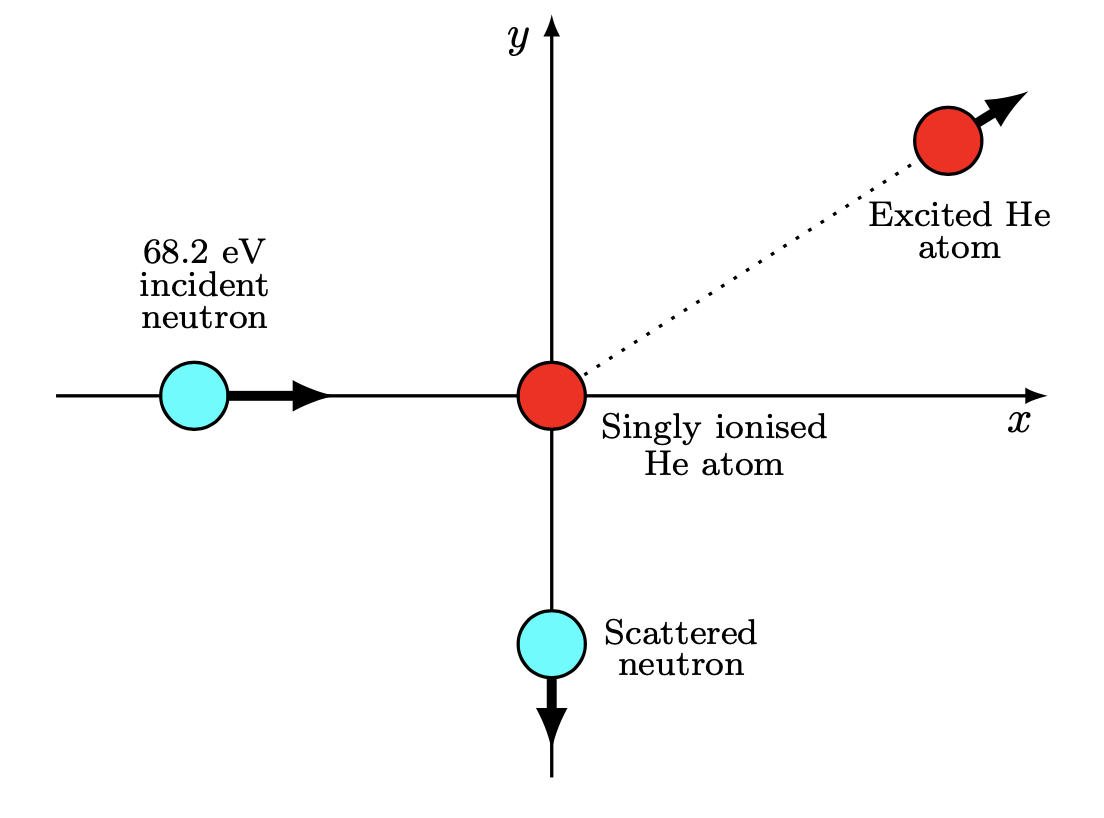
\includegraphics[width=0.5\linewidth]{spho_book_TYS_images/2018q6.png}
	\caption{}
\end{figure}

The mass of the helium atom is four times the mass of the neutron, and the energy levels of the helium atom are given by
$$
E_{n}=-\frac{54.4}{n^{2}} \mathrm{eV}
$$
i) Find the allowed values of the kinetic energies of the scattered neutron and helium atom after the collision. [8] \\
ii) If the helium atom de-excites subsequently by emitting radiation, find the range of wavelengths of the emitted radiation. For this part, you may assume that the momentum of the emitted photon is negligible. [4] \\
iii) When an atom emits a photon during a transition from the state with energy $E_{i}$ to the state with energy $E_{f}$, the energy of the photon is not exactly equal to the energy difference $E_{i}-E_{f}$. This is because the atom recoils, and part of the transition energy becomes the kinetic energy of recoil of the atom. Estimate the percentage of this energy difference that becomes the kinetic energy of the recoiling atom for the shortest wavelength case of the previous part. [2] \\
iv) Estimate the change in speed of the helium atom due to this transition. [2]

\subsection{Question 7}
7. A particle of mass $100 \mathrm{~g}$ is dropped from a height and falls vertically downward. The force due to air resistance is $-k v$, where $v$ is the speed of the particle and $k=1.09 \times 10^{-2} \mathrm{~kg} \mathrm{~s}^{-1}$ is a constant. \\
i) What is the terminal velocity of the particle? [1] \\
ii) How long does it take for the particle to achieve $99 \%$ of the terminal velocity? [4] \\
iii) How far has the particle fallen when it achieves $99 \%$ of the terminal velocity? [4]

\subsection{Question 8}
8. a) If a particle of charge $q$, mass $m$ and velocity $\mathbf{v}=v_{x} \hat{\mathbf{i}}+v_{y} \hat{\mathbf{j}}$ travels in a magnetic field $\mathbf{B}=B_{z} \hat{\mathbf{k}}$, then a Lorentz force $\mathbf{F}=F_{x} \hat{\mathbf{i}}+F_{y} \hat{\mathbf{j}}$ acts on the particle. As a result, the particle moves in a circular orbit. Assume that the particle is non-relativistic and that radiation is negligible. \\
i) Derive an expression for $T$, the time taken for the charged particle to make one complete revolution in the orbit in terms of $m, q$ and $B_{z}$. [2] \\
ii) Write down an expression for the acceleration of the particle $\mathbf{a}=a_{x}(t) \hat{\mathbf{i}}+a_{y}(t) \hat{\mathbf{j}}+a_{z}(t) \hat{\mathbf{k}}$ in terms of $v_{x}(t), v_{y}(t), v_{z}(t)$ and $T$. [3] \\
b) To compute the trajectory of the particle, we can estimate and compute the velocity of the particle after a short time step $\Delta t$, we can use a forward difference method. We assume that, to first-order, the acceleration in the $x$ and $y$-directions are constant during this short period of time such that $v_{x}(t+\Delta t) \simeq v_{x}(t)+a_{x}(t) \Delta t$ [3] \\
i) Write down the equations which determine $x(t+\Delta t)$ and $y(t+\Delta t)$ from $x(t)$ and $y(t)$ in terms of $T, B_{z}, q, m$ and $\Delta t$. [3] \\
ii) Derive an equation for the change in kinetic energy $\Delta E_{k}$ after time $\Delta t$ in terms of $T, B_{z}, q$, $m$ and $\Delta t$. [3] \\
iii) Calculate the ratio $E_{k_{f}} / E_{k_{i}}$ for $\Delta t=0.01 T$, where $E_{k_{i}}$ and $E_{k_{f}}$ are the kinetic energies at the start and end of an orbit respectively. [2]
c) Another method to compute the trajectory is to use a central difference method. We still assume that the acceleration in the $x$ and $y$-directions are constant during this short period of time $\Delta t$, but for $t>2 \Delta t$, when calculating the Lorentz force, we have instead
$$
v_{x}(t) \simeq \frac{x(t+\Delta t)-x(t-\Delta t)}{2 \Delta t} \text { and } a_{x}(t) \simeq \frac{x(t+\Delta t)-2 x(t)+x(t-\Delta t)}{\Delta t^{2}}
$$
i) Obtain equations to calculate $x(t+\Delta t)$ from $x(t)$ and $x(t-\Delta t)$, as well as $y(t+\Delta t)$ from $y(t)$ and $y(t-\Delta t)$, in terms of $B_{z}, q, m$ and $\Delta t$. [6] \\
ii) Derive an equation for the change in kinetic energy $\Delta E_{k}$ after time $\Delta t$ in terms of $B_{z}, q, m$ and $\Delta t$ via the central difference method. [4] \\
d) On the same diagram, sketch (alongside the actual trajectory of the particle) the trajectories of the particle as computed using the forward the central difference methods. [2]

\subsection{Question 9}
9. A rocket of proper length $600 \mathrm{~m}$ is moving directly away from the earth with uniform velocity. A radar pulse is sent out from the earth and is reflected from the reflectors at the back end and the front end of the rocket. The first reflected radar pulse is received back at the base $5.0$ minutes after emission and the second reflected pulse is received $12.0 \mu \mathrm{s}$ later. \\
i) Calculate the distance of the rocket from the earth at the instant the outgoing radar pulse hits the back end reflector. [2] \\
ii) Calculate the velocity of the rocket relative to the earth. [5] \\
iii) Calculate the time interval between the reflections at the back end and front end of the rocket measured in the inertial frame of the rocket. [3] \\
iv) Explain why the time interval between the reflections in the two frames (i.e. the earth frame and the rocket frame) are not related by the time dilation formula. [3]

\end{document}
